\documentclass[12pt,letterpaper]{article}
\usepackage{./preamble}
\usepackage{amsmath}

%%%%%%%%%%%%%%%%%%%%%%%%%%%%%%%%%%%%%%%%%%
%%%% Edit These for yourself
%%%%%%%%%%%%%%%%%%%%%%%%%%%%%%%%%%%%%%%%%%
\newcommand\course{Computational Statistics}
\newcommand\hwnumber{4}
\newcommand\userID{Davi Sales Barreira}
\DeclareRobustCommand{\rchi}{{\mathpalette\irchi\relax}}
\newcommand{\irchi}[2]{\raisebox{\depth}{$#1\chi$}}
\newcommand*{\QEDA}{\hfill\ensuremath{\blacksquare}}%

\begin{document}
% \textbf{\Large Worksheet completed with Octave.}

\section*{Exercise 1 (Kalma Filter)}
\begin{enumerate}[leftmargin=!,labelindent=5pt]
\item 
$$
f(X_t \mid X_{t-1}) \sim N(\phi X_{t-1}, \sigma_v^2)
$$
$$
g(Y_t \mid X_{t}) \sim N(\phi X_{t}, \sigma_w^2)
$$

\item Note that $X_{t+1} = \phi X_t + V_t$. Then:
$$
X_{t+1} \mid Y_{1:t} = \phi X_t + V_t \mid Y_{1:t}
$$
Therefore, since
$X_t \mid Y_{1:t} \sim N(m_{t\mid t}, \sigma^2_{t\mid t})$ and
$V_t \sim N(0, \sigma_v^2)$, we have the sum of normals, hence:
$$
X_{t+1} \mid Y_{1:t} \sim N(m_{t\mid t}, \sigma_v^2 +
\phi^2 \sigma^2_{t\mid t})
$$

\item Note that:
$$
p(X_{t=1} \mid Y_{1:t},Y_{t+1}) \propto
N(X_{t+1},\sigma_w^2)N(m_{t+1}, \sigma_{t+1}^2)
$$

The update of normal distribution by normal distribution is given by:
$$
\mu_1 = \frac{y_{t+1}\sigma_w ^{-2} + m_{t+1}\sigma_{t+1}^2}
{\sigma_w^{-2} + \sigma_{t+1}^{-2}}
\quad \quad
\tau_1^2 = (\sigma_w^{-2}+\sigma_v^{-2})^{-1}
$$
Hence, $p(x_{t+1} \mid y_{1:t}) = N(\mu_1, \tau_1^2) =
N(m_{t+1\mid t},\sigma^2_{t+1 \mid t})$.

\item Note that:
$$
Y_{t+1} \mid Y_{1:t} = X_{t+1} + W_{t+1} \mid Y_{1:t} =
N(\mu_1,\tau_1) + N(0, \sigma_w ^2)
$$

$$
Y_{t+1} \mid Y_{1:t} = N(\mu_1,
\sigma_w^2 + \tau_1^2)
$$

\end{enumerate}

\newpage
\section*{Exercise 2 (SIS filter)}
\begin{enumerate}[leftmargin=!,labelindent=5pt]
\item $v_t$ approximate $p(x_t \mid y_{0:t})$. Since this is the
filtering distribution, that is why it is called a filter.

\item 
$$
p_{Y_0}(y_0) = \int p_{Y_0,X_0}(y_0, x_0)dx_0
= \int p_{Y_0\mid X_0}(y_0\mid x_0)p(x_0)dx_0 = 
\int g(y_0 \mid x_0) \mu(x_0)dx_0
$$
And,
$$
p_{Y_0,X_0}(y_0, x_0) = \int p_{Y_0,X_0,X_0,Y_1}(y_0, x_0,x_1,y_1)dx_0 dx_1
= $$
$$
\int 
p_{Y_1 \mid X_0,X_0,Y_1}(y_1 \mid x_0,x_1,y_0)
p_{X_1 \mid Y_0,X_0}(x_1 \mid x_0,y_0)
p_{Y_0 \mid X_0}(y_0 \mid x_0) p_{X_0}(x_0)
dx_0 dx_1 =
$$
$$
\int 
g(y_1 \mid x_1)
f(x_1 \mid x_0)
g(y_0 \mid x_0) \mu(x_0)
dx_0 dx_1
$$

\item First, $p_{Y_0}(y_0) = E_\mu[g(Y_0 \mid X_0)] =
E_{X_0}[g(Y_0 \mid X_0)]$, hence an unbiased estimator is 
$\frac{\sum^n_{i=1} g(y_0 \mid X_0^{(i)})}{n}$, which is an estimation
for the expected value.

Now, $p_{Y_0,Y_1}(y_0, y_1) = E_{X_0,X_1}[g(y_1 \mid x_1)g(y_0 \mid x_0)]$,
hence we have the unbiased estimator equal to 
$\frac{\sum^n_{i=1} g(y_0 \mid X_0^{(i)})
g (y_1 \mid X_1^{(i)})}{n}$.

\item
\item 
\item 
\end{enumerate}



\newpage
\section*{Simulation question (Reversible jump MCMC)}
The model samples
$$
\pi(\theta \mid k=1) = exp(-\theta^2/2)
\quad \quad
\pi(\theta \mid k=2) = exp(-(\theta_1^2 + \theta_2^2)/2)
$$
The analytical rate of visits of $\frac{k=2}{k=1}$
is given by $\sqrt{2\pi} \approx 2.51$.

    \begin{figure}[H]
        \centering
        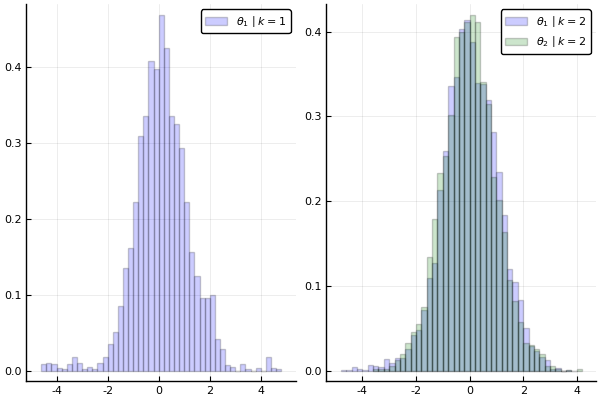
\includegraphics[width=10cm]{images/Reversible.png}
        \caption{Distribution of $\theta$ for each model. The jump
        probability used was 0.1. The distribution for $u$ was a
        standard Cauchy distribution.
        The proportion
        of visits found is 2.47.}
    \end{figure}

    \begin{figure}[H]
        \centering
        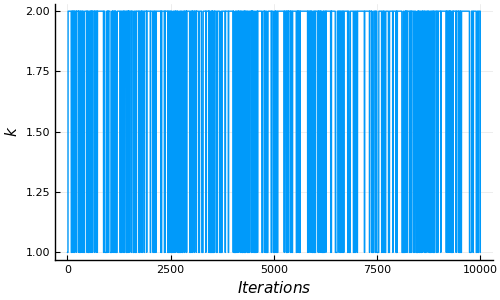
\includegraphics[width=10cm]{images/Jumps.png}
        \caption{Trace plot of the model sampled. It shows that both
        models are well sampled.}
        
    \end{figure}

\newpage
\section*{Simulation question (Reversible jump MCMC)}

The target distribution is $\pi(x) \approx exp(-10(x-1)^2)$.
The tempered distributions are shown in the graph below.

    \begin{figure}[H]
        \centering
        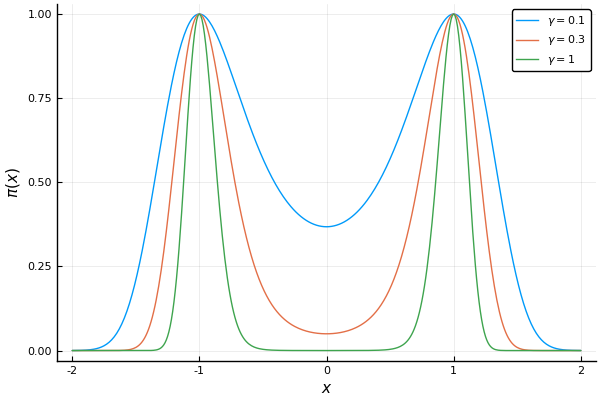
\includegraphics[width=10cm]{images/Tempered.png}
        \caption{Tempered distributions.
        }
    \end{figure}


Looking at the trace plot, for the distributions
with higher $\gamma$ we 
won't get a very good mixture. This problem is not
present when $\gamma$ is lower.

    \begin{figure}[H]
        \centering
        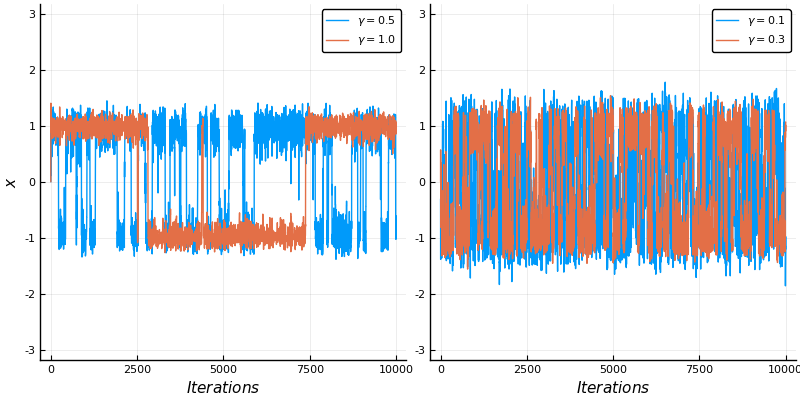
\includegraphics[width=16cm]{images/Trace1.png}
        \caption{Trace plot for different values of tempering.}
    \end{figure}

Implementing the \textit{parallel tempering}, this problem is solved as
can be seen in the figure below.

    \begin{figure}[H]
        \centering
        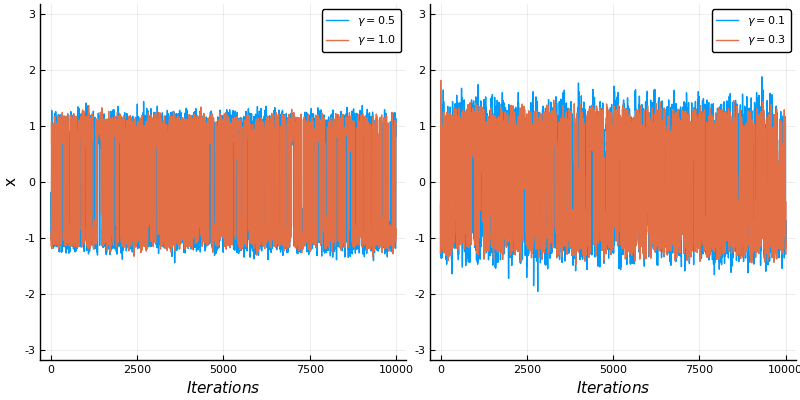
\includegraphics[width=16cm]{images/Trace2.png}
        \caption{Trace plot for the \textit{parallel tempering} model.}
    \end{figure}


\newpage
\section*{Simulation question (linear Gaussian model - SIS and SIR)}

The model is
$$
X_t = \phi X_{t-1} + \sigma_V V_t,
\quad \quad
Y_T = X_t + \sigma_W W_t,
\quad \quad
\phi = 0.95,\quad \sigma_V = 1, \quad \sigma_W = 1
$$
    \begin{figure}[H]
        \centering
        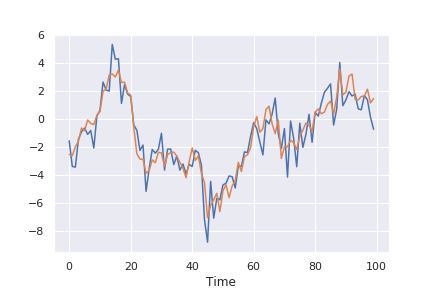
\includegraphics[width=12cm]{images/LinearGaussian.png}
        \caption{$T = 100$ simulated observations for the Linear Gaussian
        model.}
    \end{figure}

Using the prior as a proposal, we implement the sequential
importance sampling algorithm.
The results are shown below.

    \begin{figure}[H]
        \centering
        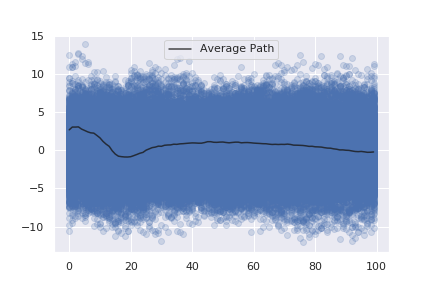
\includegraphics[width=12cm]{images/SIS_Paths.png}
        \caption{Simulated particles for N = 1000 using SIS.}
    \end{figure}

    \begin{figure}[H]
        \centering
        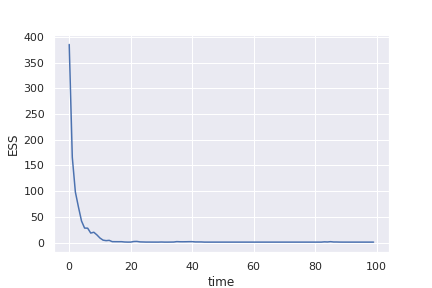
\includegraphics[width=12cm]{images/ESS_SIS.png}
        \caption{Effective sample size.}
    \end{figure}
    Looking at the effective sample size we immediatly notice
    the problem with the SIS algorithm. The effective sample size
    quickly drops.

    Now let's show the SIR algorithm and how this problem is solved.
    \begin{figure}[H]
        \centering
        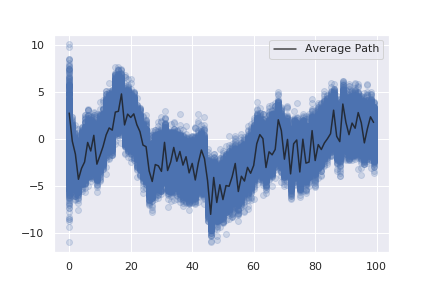
\includegraphics[width=12cm]{images/SIR_Paths.png}
        \caption{Simulated particles for N = 1000 using SIR.}
    \end{figure}

    \begin{figure}[H]
        \centering
        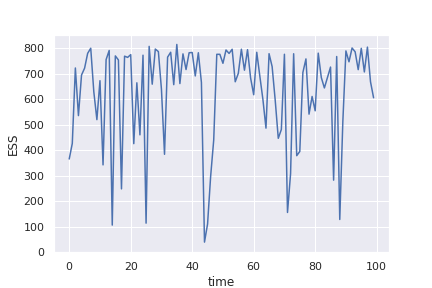
\includegraphics[width=12cm]{images/ESS_SIR.png}
        \caption{Effective sample size.}
    \end{figure}


\end{document}
